\chapter{Introduction}
Radiology is a powerful tool to detect and diagnose abnormalities by allowing doctors to visually inspect internal pathology that could not otherwise be seen. By virtue of integrating a ubiquitous medical practice with sophisticated engineering, the field has traditionally been at the forefront of medical technology. Digital radiology and picture archiving and communications systems led to an early, widespread adoption of electronic records with respect to imaging \cite{Strickland:2000cv,Bryan:1999kn}.

Despite the early adoption of computational systems to manage data, the actual practice of radiology remains a relatively unchanged. The doctor must still visually scan, detect, and interpret the findings in the image to deliver an impression. An unfortunate consequence of such a system is substantial variability in practice and performance \cite{Robinson:1997uq,Fitzgerald:2001hn}. This is not to say that radiologists are the only doctors faced with these issues, as the now infamous Institute of Medicine report \emph{To Err is Human: Building a Safer Health System} revealed a striking amount of poor patient outcomes are a result of medical error \cite{Anonymous:2000va}. A prominent recommendation from this study is the use of automation and computation to improve upon standard of care via decision support systems.

Decision support systems are tools that incorporate medical information to provide meaningful input to medical practitioners. They have been developed for a large variety of domains in medicine \cite{Bright:2012ga,Garg:2005cb,Miller:1994cx,Kawamoto:2005gn}. Despite significant technological achievements, adoption of these systems in radiology is limited as they often interrupt the  work-flow \cite{Morgan:2011ct}. In addition, current radiological decision support is mainly focused on diagnosis and automated computational analysis of image data \cite{Garg:2005cb, Burnside:2000wl, ElizabethS:2005gc, Rubin:2005jg} - the so-called \emph{Greek Oracle} model of decision support \cite{Miller:1990wg,Miller:1994cx}. Such systems have been shown to fail when deployed in practice since they are based on the implicit assumption that computers can perform the duties of doctors better than doctors themselves. Charles Friedman goes so far as to declare that the \emph{Fundamental Theorem of Biomedical Informatics} is that decision support should ``augment human reasoning'' beyond the capabilities of an unaided practitioner \cite{Friedman:2009dx}. Thus, it is crucial to develop radiological decision support tools that fit into the work-flow and augment their reasoning. A perfect window to provide this is during radiological reporting \cite{Noumeir:2006cb}.

The report is of crucial importance, since it conveys the radiologist findings, interpretation of those findings, and suggested patient management. It is frequently the primary form of communication between radiologists and referring clinicians or patients \cite{Sistrom:2005cx}. Improvement of reporting directly improves such communication and indirectly may improve the radiologist's own performance. Prior studies have shown the importance of good reporting practices and identified several key traits of good reports: correctness of findings, completeness of the description of significant clinical findings, consistency of report language and findings, and timeliness of the report's completion \cite{Johnson:2004kh, HaraldO:2004hi}.

Considerable effort has been made to improve upon the variability in report content and diagnosis; arguably the most successful of which is in mammography \cite{Langlotz:2009fn,Burnside:2009ki}. The Breast Imaging-Reporting and Data System (BI-RADS) provides a standard lexicon of descriptors for radiological observations \cite{Liberman:ws}. This standardized language has virtually eliminated ambiguity in terminology across the United States. Further work has been done to create the RadLex ontology for a more universal solution to radiological terminology \cite{Langlotz:2006jn}. Yet, there is still a substantial body of work revealing variability with regard to sensitivity and specificity of evaluation of lesion malignancy amongst different readers as well as different facilities \cite{Jackson:2009fw, Beam:1996ui, Elmore:2002vc, Taplin:2008bv}. Such variability is not restricted to diagnosis and impressions; even the \emph{findings} within the contents of the report have shown variability \cite{Hobby:2000th, Robinson:1997uq}.

Another solution to improving upon radiological reports is the use of \emph{Structured Reporting Systems}. Such systems provide templates with standardized information and structure as well as support for terminologies like RadLex or BI-RADS \cite{Reiner:2009ib}. Unfortunately, structured reporting is not without its drawbacks. It is generally more time-intensive and imposes distractions in the traditional radiological workflow, directly interfering with timeliness \cite{Weiss:2008er}.

Both standardized terminology and structured reports are solid steps to improving upon the reporting process, but they do not directly analyze the radiological concepts being communicated. Borrowing from the \emph{meaning triangle}, the tools described encode radiological objects with standard expressions, but they do not encode their sense or concept. Such work would need to perform higher order analysis of the information in the report including, but not limited to, analyzing if the contents in the reports is correct, complete, or even consistent with diagnosis. In this sense, decision support systems provide the missing piece for this analysis.

Our hypothesis is that improving the correctness, consistency, and completeness of radiology reports can improve the sensitivity and specificity of diagnosis and thereby improve the quality of patient care. To tackle this challenge and to enable translation of decision-support system into clinical practice to benefit patient care, we propose a real-time decision-support system that provides feedback to radiologists as they generate their reports. This system will create evaluate and improve upon the content of a structured radiological report. This differs from traditional approaches to decision-support system because our system will improve upon reporting, and by our hypothesis, implicitly improve upon practice. By ensuring that the relevant observations are correctly, completeley, and consistently described in mammography reports, our decision-support system will reduce variability in practice, improving practitioner decision making and lead to better patient care.

\section{FASR: Fast Adaptive Structured Reporting}
The Fast Adaptive Structured Reporting (FASR) system's goal is to reduce variability and error in radiological interpretation by providing decision-support during reporting time. This works by incorporating multiple checks during the reporting process and providing real-time feedback to the radiologist.

There are three main components to FASR: (1) Verification of the annotation correctness, (2) assessment of report completeness, and (3) providing feedback to the radiologist.

\begin{figure}[h]
	\centering
	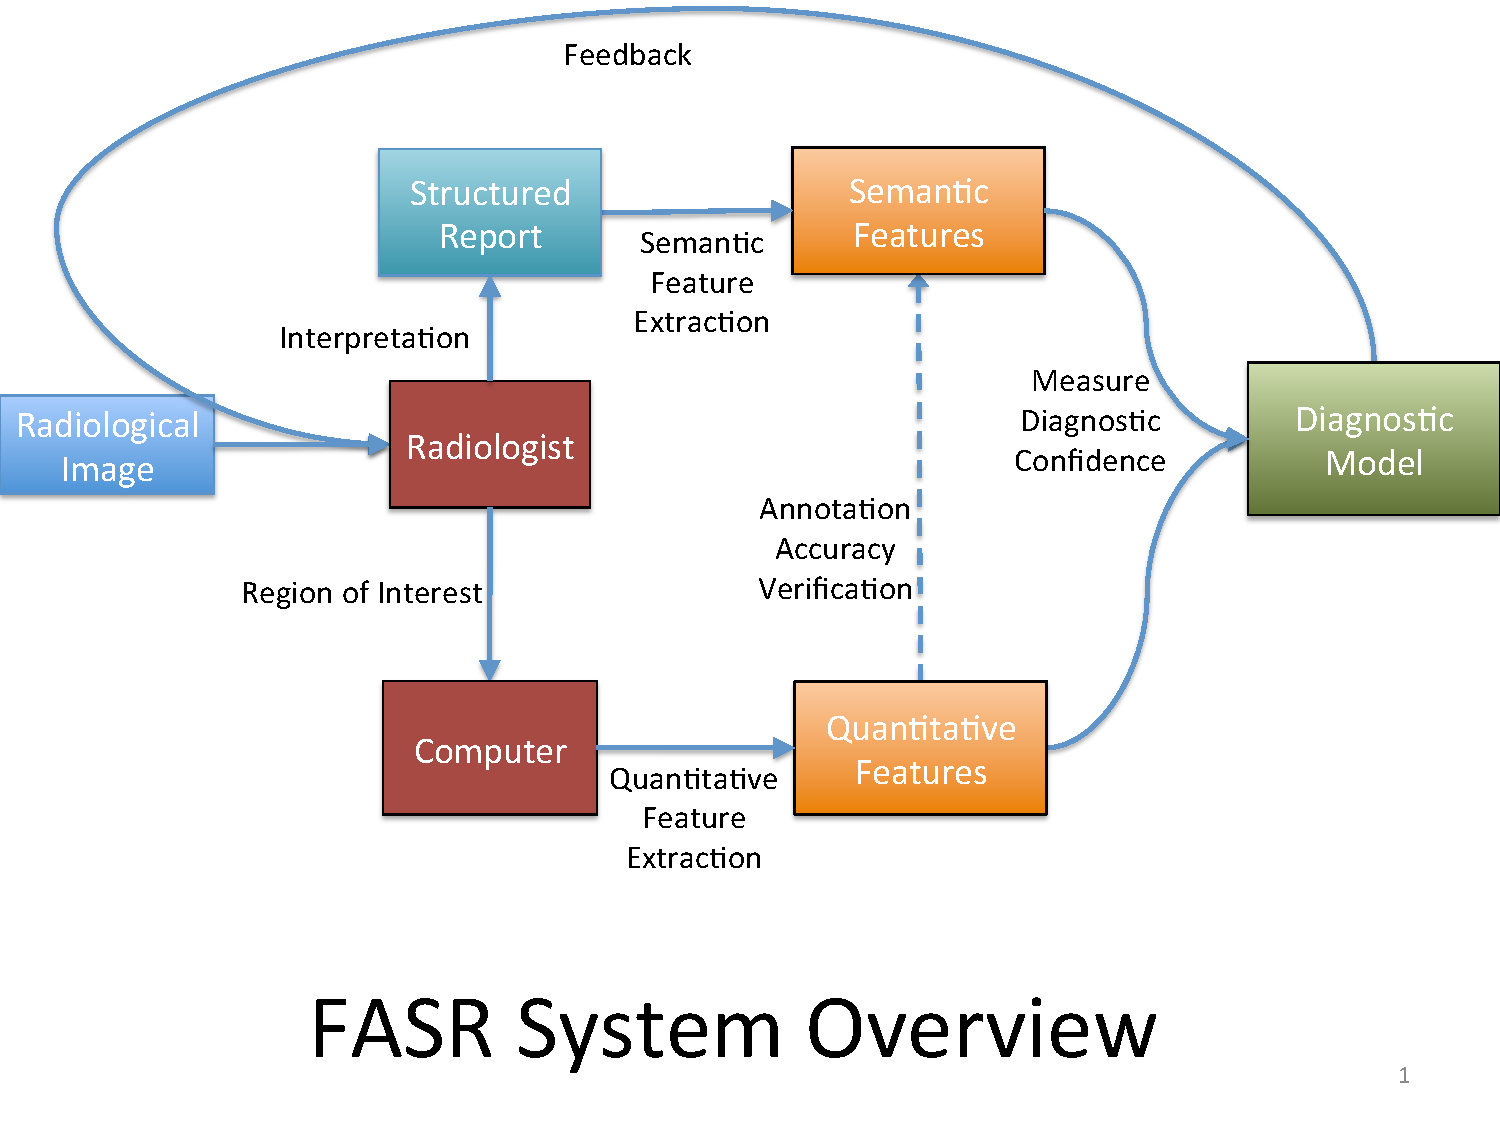
\includegraphics[width=1\linewidth]{fasr_diagram.pdf}
	\caption{Overview of the Fast Adaptive Structured Reporting (FASR) system}
	\label{fig:fasr_diagram}
\end{figure}
